
\section{TikZ Styles}

The following shows the different line widths you can use when drawing in TikZ. This should be an optional argument to the draw command.


\begin{figure}[H]
\centering
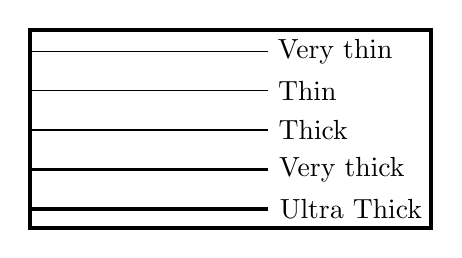
\begin{tikzpicture}[yscale=0.5]
\draw[very thin] (0,0) -- (3,0) node[right] {Very thin};
\draw[thin] (0,-1) -- (3,-1) node[right]{Thin};
\draw[thick] (0,-2) -- (3,-2) node[right]{Thick};
\draw[very thick] (0,-3) -- (3,-3) node[right]{Very thick};
\draw[ultra thick] (0,-4) -- (3,-4) node[right]{Ultra Thick};

\draw[ultra thick] (current bounding box.north east) rectangle (current bounding box.south west);

\end{tikzpicture}
\caption{Line Widths}
\end{figure}

%------------------

\begin{figure}[H]
\centering
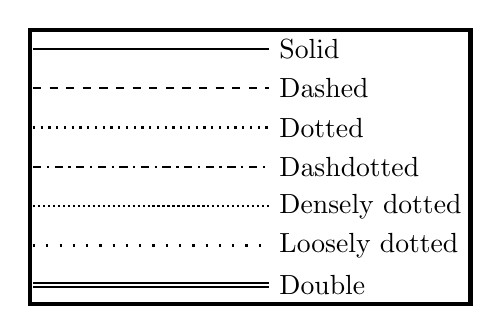
\begin{tikzpicture}[yscale=0.5]

\draw[thick,solid] (0,0) -- (3,0) node[right]{Solid};

\draw[thick,dashed] (0,-1) -- (3,-1) node[right]{Dashed};

\draw[thick,dotted] (0,-2) -- (3,-2) node[right]{Dotted};

\draw[thick,dashdotted] (0,-3) -- (3,-3) node[right] {Dashdotted};

\draw[thick,densely dotted] (0,-4) -- (3,-4) node[right] {Densely dotted};

\draw[thick,loosely dotted] (0,-5) -- (3,-5) node[right] {Loosely dotted};

\draw[thick,double] (0,-6) -- (3,-6) node[right] {Double};

\draw[ultra thick] (current bounding box.north east) rectangle (current bounding box.south west);
\end{tikzpicture}
\caption{Line Styles}
\end{figure}

%------------------
\begin{figure}[H]
\centering
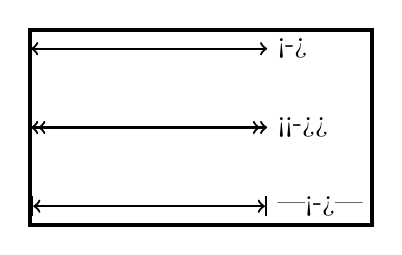
\begin{tikzpicture}[thick]
\draw[<->] (0,0) -- (3,0) node[right]{\lstinline{<->}};

\draw[<<->>] (0,-1) -- (3,-1) node[right]{\lstinline{<<->>}};

\draw[|<->|] (0,-2) -- (3,-2) node[right]{\lstinline{|<->|}};

%\draw[-*] (0,-3) -- (3,-3) node[right]{\lstinline{-*}};

\draw[ultra thick] (current bounding box.north east) rectangle (current bounding box.south west);
\end{tikzpicture}
\caption{Arrow Head Types}
\end{figure}



%------------------
\begin{figure}[H]
\centering
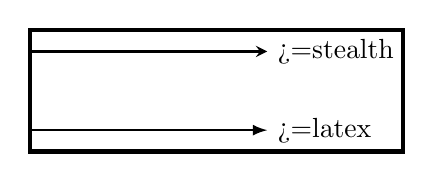
\begin{tikzpicture}[thick]

\draw[->,>=stealth] (0,0) -- (3,0) node[right]{\lstinline{>=stealth}};

\draw[->,>=latex] (0,-1) -- (3,-1) node[right]{\lstinline{>=latex}};


\draw[ultra thick] (current bounding box.north east) rectangle (current bounding box.south west);
\end{tikzpicture}
\caption{Arrow Header Styles}
\end{figure}


%% Rotational Circular Geometry

Figure \ref{Fig:rotationalcirculargeometry} shows rotational circular geometry typically seen in \textit{Dynamics}, drawn in TikZ.

\begin{figure}[H]
\centering
\begin{tikzpicture}[xscale=0.8,yscale=0.8]
% draw circle
\shadedraw[inner color=gray!10,outer color=gray!40, draw=black, very thick] (0,0) circle (3cm);


\def\y = -45 + 90
\def\z = 90 - 45

\draw[guide] (0,0) -- (\y:4cm);
\draw[guide] (0,0) -- (-45:5cm);
\draw[guide] (0,0) -- (5,0);

% phi-theta
\draw[->, very thick, blue] (5,0) arc (0:\z:5cm) node[label] {$\phi-\theta(t)$};

% phi
\draw [<-, very thick, space] (\y:4cm) arc (\y:-45:4cm) node[label] {$\phi$};

% theta
\draw[->, very thick] (5, 0) arc (0:-45:5cm) node[label] {$\theta(t)$};

% base vectors
%\draw[basevec] (\z:4cm) -- (\z:5cm);
%\draw[basevec] (\z:4cm) -- +(\z+90:1cm);
\nandm{45:4cm}{45}

% Points of interest
\poi{0,0}
\poi{-45:4cm}
\poi{5,0}

\end{tikzpicture}
\caption{Rotational Circular Geometry}
\label{Fig:rotationalcirculargeometry}
\end{figure}

% Rotate around
% Scope trick.
% https://tex.stackexchange.com/questions/19284/problem-when-drawing-an-axis-aligned-bounding-box-around-a-tilted-rectangle

Figure \ref{Fig:platonpin} shows how the idea of a \textit{scope} can be used to rotate objects in that scope about a point.

\begin{figure}[H]
\centering
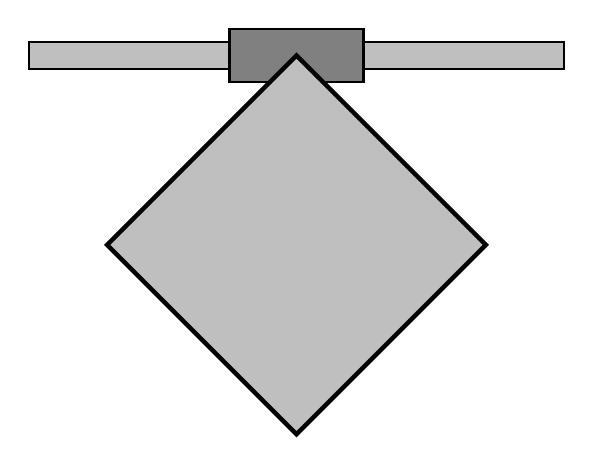
\begin{tikzpicture}[scale=1.7]
\centering

\shadedraw[top color=lightgray,middle color=gray,bottom color=lightgray,thick] (-2,-0.1) rectangle (2,0.1);
\draw[thick,fill=gray] (-0.5,-0.2) rectangle (0.5,0.2);

\begin{scope}[rotate around={-135:(0,0)}]
\draw[ultra thick,fill=lightgray] (0,0) rectangle (2,2);
\end{scope}
\poi{0,0}
%\poi{2,2}

\end{tikzpicture}
\caption{Rotating plate connected to pin}
\label{Fig:platonpin}
\end{figure}


Figure \ref{Fig:mulispringsys} is a multi-spring system drawn with TikZ. The springs are rendered using the \textit{stanli} package. The package offers a spring lifestyle.

% https://tex.stackexchange.com/questions/430943/latex-stanli-package-how-to-design-a-spring-element#430951
\begin{figure}[H]
\centering
\begin{tikzpicture}

\draw[thin,fill=lightgray] (0,-0.1) rectangle (9,0.1);

\begin{scope}
\draw[ultra thick,fill=gray] (2,-0.5) rectangle (3,0.5);
\draw[spring] (0,0) -- (2,0);
\end{scope}

\begin{scope}[xshift=3cm]
\draw[ultra thick,fill=gray] (2,-0.5) rectangle (3,0.5);
\draw[spring] (0,0) -- (2,0);
\end{scope}

\begin{scope}[xshift=6cm]
\draw[ultra thick,fill=gray] (2,-0.5) rectangle (3,0.5);
\draw[spring] (0,0) -- (2,0);
\end{scope}

%\filldraw[shading=axis,top color=gray, bottom color=white,line width=10pt, cap=round] (0,-1) --(2,-1);

\end{tikzpicture}
\caption{Drawing springs}
\label{Fig:mulispringsys}
\end{figure}


\begin{figure}
\centering
\begin{tikzpicture}[scale=2,decoration={
	markings,% switch on markings
	mark=% actually add a mark
	between positions 0 and 1 step 2.5mm with
{
	\begin{scope}[rotate around={110:(0,0)}]
		\shadedraw[rounded corners=0.2pt,
			right color=gray,
			left color= gray,
			middle color=white,
			line width=0
			]
		(-2pt,-0.5pt)
		rectangle
		(8pt,0.5pt);
	\end{scope}
	\begin{scope}[xshift=2pt,rotate around={72:(0,0)}]
		\filldraw[rounded corners=0.5pt, color=gray,fill=gray]
		(-1.5pt,-0.5pt)
		rectangle
		(7.5pt,0.5pt);
	\end{scope}
}
}
]
\draw [help lines] grid (3,2);
\draw [postaction={decorate}] (0,0) -- (2,0);
\end{tikzpicture}
\end{figure}



\begin{figure}
\centering
\begin{tikzpicture}[scale=2,decoration={
	markings,% switch on markings
	mark=% actually add a mark
	between positions 0 and 1 step 2.5mm with
{
	\begin{scope}[rotate around={110:(0,0)}]
		\shadedraw[rounded corners=0.2pt,
			right color=gray,
			left color= gray,
			middle color=white,
			line width=0
			]
		(-2pt,-0.5pt)
		rectangle
		(8pt,0.5pt);
	\end{scope}
	\begin{scope}[xshift=2pt,rotate around={72:(0,0)}]
		\filldraw[rounded corners=0.5pt, color=gray,fill=gray]
		(-1.5pt,-0.5pt)
		rectangle
		(7.5pt,0.5pt);
	\end{scope}
}
}
]
\draw [help lines] grid (3,2);
\draw [postaction={decorate}] (0,0) -- (2,0);
\end{tikzpicture}
\end{figure}










